        \clearpage
        \begin{figure*}[ht]
            \pdfbookmark[2]{ID 05}{figure_id_05}
        	\centering
            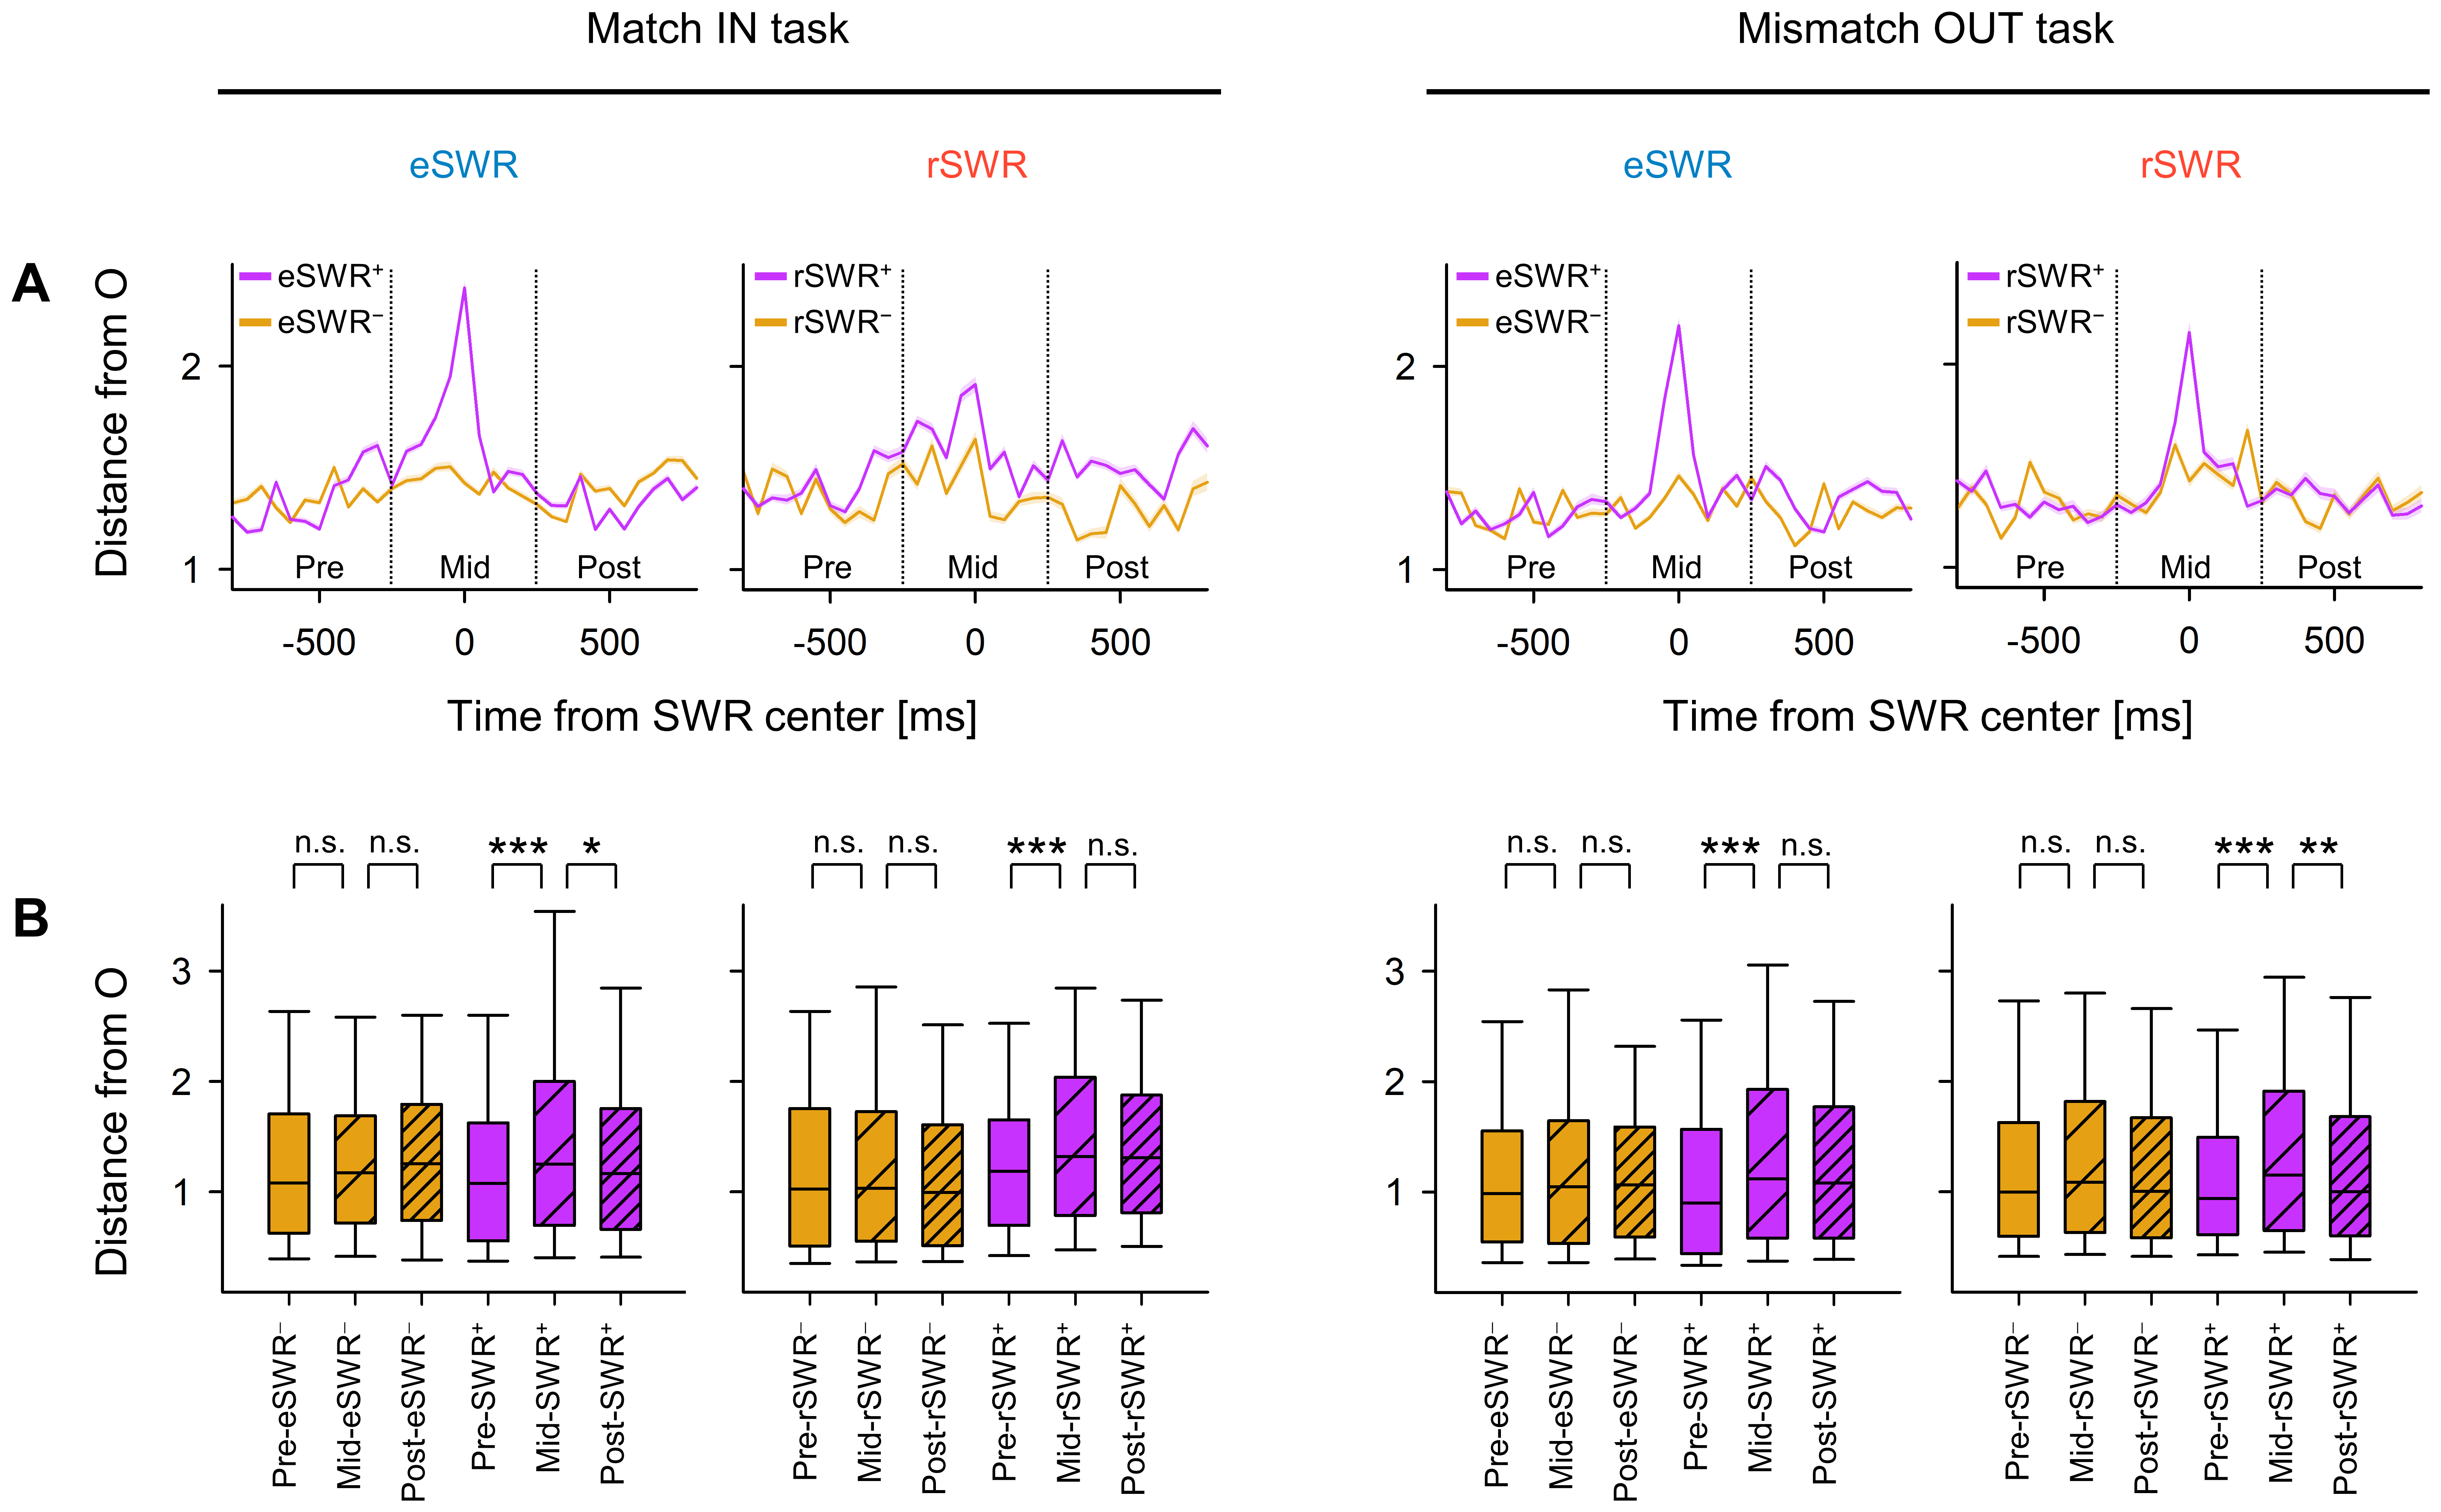
\includegraphics[width=1\textwidth]{./src/figures/.png/Figure_ID_05.png}
        	\caption{\textbf{
Transient neural trajectory change during SWR
}
\smallskip
\\
\textbf{\textit{A.}} Distance from the origin ($O$) of the peri-sharp-wave-ripple trajectory (mean \textpm 95\% confidence interval; however, the interval may not be easily visible due to the narrow range.).  \textbf{\textit{B.}}  The distance from the origin during the mid-SWR$^+$ period was found to be longer compared to the corresponding pre-SWR$^+$ period (*\textit{p} $<$ 0.05, **\textit{p} $<$ 0.01, ***\textit{p} $<$ 0.001; Brunner--Munzel test). Abbreviations: SWR, sharp-wave ripple events; eSWR, SWR during the encoding phase; rSWR, SWR during the retrieval phase, SWR$^+$, SWR event; SWR$^-$ control events for SWR$^+$; pre-SWR, mid-SWR, or post-SWR, the time interval from $-800$ to $-250$ ms, from $-250$ to $+250$ ms, or from $+250$ to $+800$ ms from the center of SWR.
}
% width=1\textwidth
        	\label{fig:05}
        \end{figure*}
